% !TeX root = ../main.tex
% -*- coding: utf-8 -*-


\chapter{技术背景} 
\label{2}

引言

\section{深度神经网络及相关术语}

人工神经网络是一种类似于人类大脑生物神经系统的信息处理模型,它由许多相互连接的神经元(网络中的节点)组成,这些神经元都可以向其他神经元发送信号。一般的神经网络由输入层,隐藏层和输出层组成,如图\ref{深度神经网络结构图}所示,如果一个神经网络有多个隐藏层,那么这个神经网络就被称为深度神经网络。DNN的隐藏层一般由卷积层,池化层,全连接层,Dropout层和Softmax层构成,数据输入输入层后,会经过每一层,每层提取的抽象特征会作为下一层的输入,最终由输出层输出。

\begin{figure}[htbp]%%图,[htbp]是浮动格式
	\centering
	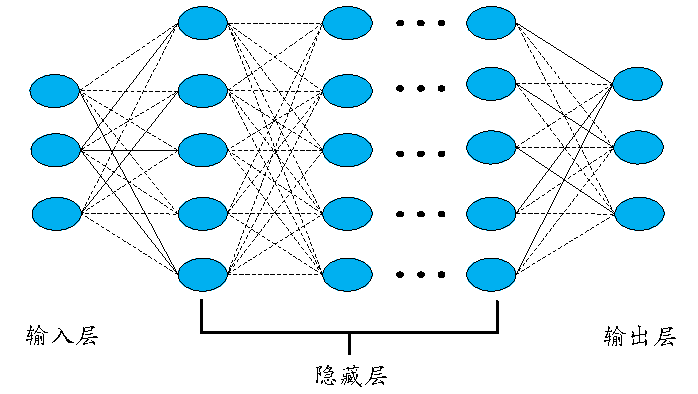
\includegraphics[width=11cm,height=7cm]{深度神经网络结构.pdf}
	%	\centerline{原始样本}
	\setlength{\abovecaptionskip}{5mm} %图片标题与图片距离
	\caption{深度神经网络结构图}
	\label{深度神经网络结构图}
\end {figure}

DNN可以看作是将一组输入变量转化为一组输出变量的非线性数学函数。每个神经元都有对应的权重和偏置参数,控制着输入的精确转化,这些参数在反向传播的过程中,通过损失函数和梯度下降算法来更新。确定这些参数的过程称为DNN模型的学习或者训练,并且需要大量的计算资源,然而权重一旦确定,DNN模型就可以快速的处理相似类型的新数据,识别并提取海量数据中的复杂特征。

以下是本文中涉及到DNN知识产权保护领域中的相关术语:

\begin{enumerate}
	\renewcommand{\labelenumi}{\theenumi)}
	\item 源模型。源模型也称作目标模型,是指模型所有者在私有或公共数据集上,消耗大量计算资源和人力资源训练出的高性能DNN模型,可能因学术研究放置在开源社区,或者作为商用给用户提供远程API。
	\item 可疑模型。可疑模型是指该模型可能是通过模型窃取攻击方法从源模型派生出来的模型,判断一个可疑模型是否是从源模型派生是模型知识产权保护领域的主要目标。
	\item 白盒模式。白盒模式是指能够获得DNN模型的所有知识,包括训练集,训练方式,模型参数,模型结构等。
	\item 黑盒模式。黑盒模式指不清楚模型内部参数,但可以通过模型提供的API获得指定输入的输出。
\end{enumerate}



\section{对抗性攻击}

\subsection{对抗性样本}
 
对抗性样本的概念是Szegedy等人\cite{szegedy2013intriguing}提出的。这篇文章中指出,通常情况下,一个良好性能的DNN模型具备很好的泛化能力,对输入的随机微小扰动具有鲁棒性,因此小扰动不应该改变图像的预测类别。然而,对图像添加特定的非随机扰动,使得损失函数的值增大,可以任意改变DNN模型的预测结果。这种人类肉眼上难以察觉但可以使模型输出错误类别的样本称为对抗性样本。 

用$f:R^m \rightarrow {1,2,...,n}$表示将一张图片映射为$n$个标签的DNN分类器,对一个正常样本$x \in R^m$以及一个错误标签$l$,目标是找到一个最小的扰动$\delta$,使得分类器将样本$x$错误分类为$l$,如式\ref{eq:1}所示:
\begin{equation}
	\label{eq:1}
	\begin{split}
	&min\parallel \delta \parallel_2, \\
	 &s.t. \ f(x + \delta) = l,\ x + \delta \in [0,1]^m
	\end{split}
\end{equation}
其中叠加了扰动的$x +\delta$即为一个对抗性样本。\ref{eq:1}这种方式通常用在黑盒的场景下,仅根据DNN分类器的输出进行扰动$\delta$的调整。
 
 在白盒场景下,由于知道模型的所有知识,可以根据这些信息来寻找对抗性样本,通常利用DNN分类器的损失函数来寻找对抗性样本。
 
 用$f:R^m \rightarrow {1,2,...,n}$表示将一张图片映射为$n$个标签的DNN分类器,对一个正常样本$x \in R^m$以及它对应的正确标签$y$,目标是找到一个足够小小的扰动$\delta:\delta \leq \gamma$,使得加上扰动后的样本输入DNN模型后,损失函数$L$达到最大值,如式\ref{eq:2}所示:
 \begin{equation}
 	\label{eq:2}
 		\delta = arg \mathop{max} \limits_{\delta \leq \gamma} L(f(\theta, x + \delta), y)
\end{equation}
其中$\theta$是分类器$f$的参数,$x + \delta$是一个扰动后的对抗性样本。
 
 \subsection{对抗性攻击的类别}

对抗性攻击技术是指生成对抗性样本的方法,不同的方法生成对抗性样本的效率,质量也不相同。根据方式的不同,可以分为以下几类:

\begin{enumerate}
	\renewcommand{\labelenumi}{\theenumi)}
	\item 白盒攻击与黑盒攻击。白盒攻击指敌手知道DNN模型的参数和内部结构等信息,利用这些信息发起的攻击。黑盒攻击指敌手仅根据模型的输入输出来发起攻击。
	\item 有目标攻击和无目标攻击。有目标攻击指对抗性样本的预测类别为敌手指定的类别,例如将一张牛的图片识别为羊,而不能是其他类别,常采取的方式是向各个方向搜索扰动来最大化DNN模型预测特定类上的可能性。无目标攻击指添加扰动来改变原始预测类别,对具体分类类别不做要求。通常来说有两种攻击方式,一种是最小化DNN模型预测正确类的可能性,一种是进行多次不同类别的的有目标攻击,然后在多个对抗性样本中选取扰动最小的。
	\item 单步攻击和迭代攻击。单步攻击指通过一次添加扰动生成对抗性样本,迭代攻击指通过多次迭代添加微小扰动来生成对抗性样本。通常来说迭代攻击的成功率较高,但是相应的算法复杂度更高,效率较低。
	\item 个体攻击和普适性攻击。个体攻击指针对每个样本都需要重新生成扰动,普适性攻击指找到一个通用的扰动,对数据集中的一类数据都叠加该扰动,普适性攻击效率较高,但是寻找通用扰动的难度较大。
\end{enumerate}

\section{生成对抗网络}

Goodfellow等人\cite{goodfellow2014generative}第一次提出了生成对抗网络(Generative Adversarial Network, GAN),GAN由一个生成器和一个判别器构成,

\begin{figure}[htbp]%%图,[htbp]是浮动格式
	\centering
	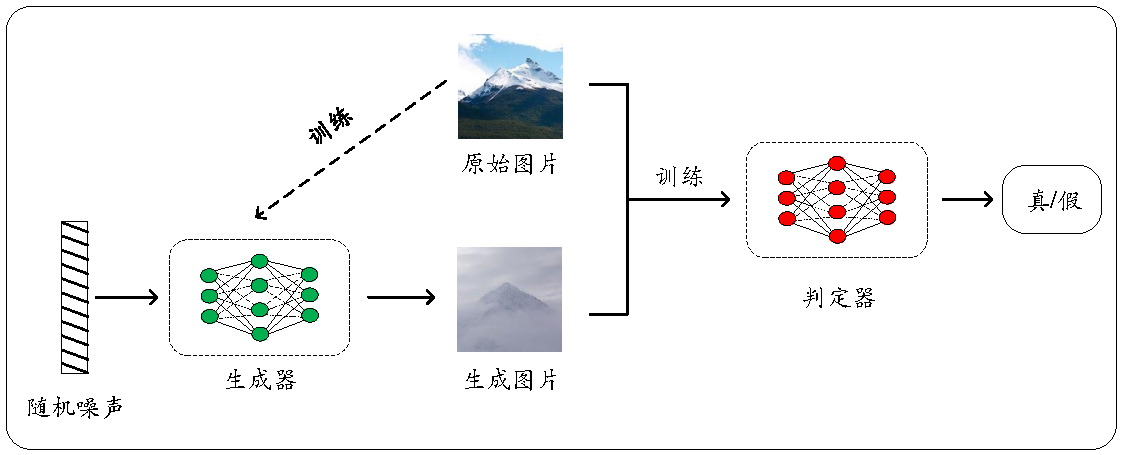
\includegraphics[width=14.5cm,height=7cm]{生成对抗网络结构.pdf}
	%	\centerline{原始样本}
	\setlength{\abovecaptionskip}{5mm} %图片标题与图片距离
	\caption{生成对抗网络结构图}
	\label{生成对抗网络结构图}
\end {figure}






\section{深度神经网络模型窃取攻击}

深度神经网络模型窃取攻击相关概念


\section{深度神经网络模型的知识产权保护}


深度神经网络模型的知识产权保护相关概念


\section{本章小结}


小结
